\pagestyle{headings}
\chapter{Continuous Random Variables} \label{chp 4}
\thispagestyle{fancy}

\subsection*{Introduction: Waiting For Dinner}
Alice and Bob arrive home from work at independently determined random times between 5:00\,pm and 6:00\,pm. How long, on average, does the person who arrives earlier spend waiting for the one who arrives later?
\par
If we measure Alice's arrival time in hours after 5:00\,pm, then it can take any value in the interval $[0,1]$. The same is true for Bob's arrival time, and the difference between the two arrival times. Random variables such as these which can take any value in an interval $I \subseteq \mathbb{R}$ are the subject of this chapter.
\par
We can represent a pair of arrival times using a point in the unit square, with Alice's arrival time determining the horizontal coordinate, and Bob's determining the vertical coordinate. If Alice arrives first, the horizontal coordinate is smaller, so the point lies above the diagonal, and the time Alice must wait for Bob to arrive is the vertical distance to the diagonal (can you explain why?).
\begin{center}
\begin{tikzpicture}[scale=0.7]
\node (v1) at (-0.75,0) {};
\fill (v1) circle [radius=2pt];
\node (a) at (-1.8,-1.8) {$0$};
\node (b) at (1.8,-1.8) {$1$};
\node (c) at (-1.8,1.8) {$1$};
\node (l1) at (1.5,1.5) {};
\node (l2) at (-1.5,-1.5) {};
\draw[dotted] (l1.center) -- (l2.center);
\draw(v1.center) -- (-0.75,-0.75);
\draw (-1.5,-1.5) rectangle (1.5,1.5);
\end{tikzpicture}
\end{center}
Similar remarks apply if Bob arrives first, in which case the time Bob must wait for Alice to arrive is the horizontal distance to the diagonal from the point representing the pair of arrival times.
\par
Therefore, the solution to our problem is the average distance between a point in the unit square and the diagonal of the unit square, where we measure distance by moving only vertically or horizontally. At the moment, calculating this average is a daunting prospect. We need to develop the fundamentals of random variables that take values in intervals, and then we'll finish this problem in Section \ref{UniformDistSec}. 

\section{Continuous Probability Distributions} \label{sec 4.1}

In Section \ref{sec 3.1}, we defined a random variable as a function from $\Omega$ to $\mathbb{R}$, but in the chapter that followed, we only dealt with random variables that take values in some discrete subset $A \in \mathbb{R}$. We saw that we could specify the distribution of a random variable using either a table, a probability mass function, or a cumulative distribution function.
\par
Our goal is now to understand what happens when a random variable can take any value in some interval $I \in \mathbb{R}$. Consider for example a random variable $X$ which represents a number chosen at random from the interval $[0,1]$.
\par
It's not possible to write the distribution of $X$ as a table, since $[0,1]$ is not a discrete set, that is, we can't write $[0,1]$ as a list. Moreover, we saw in Section \ref{ProbInterpretationSection} that for any $r \in [0,1]$, the probability $X$ will take precisely that value is zero, so if we define the probability mass function of $X$ as we did in Chapter \ref{chp 3}, the resulting function is zero everywhere, so the pmf is no longer a useful notion.
\par
Fortunately, the cumulative distribution function comes to the rescue. What is $P(X \leq \frac{2}{3})$? If we divide the interval into thirds, then $X \leq \frac{2}{3}$ when $X$ falls into one of the left two thirds, which should happen two thirds of the time if $X$ is equally likely to fall anywhere in $[0,1]$.
\vspace{0.5em}
\begin{center}
\begin{tikzpicture}
\draw (0,0) -- (3,0);
\draw[shift={(0,0)},color=black] (0pt,3pt) -- (0pt,-3pt);
\draw[shift={(3,0)},color=black] (0pt,3pt) -- (0pt,-3pt);
\foreach \x in {1,2}
\draw[shift={(\x,0)},color=black] (0pt,0pt) -- (0pt,-3pt) node[below] 
{$\frac{\x}{3}$};
\draw (0,-0.2) node[below]{$0$};
\draw (3,-0.2) node[below]{$1$};
\fill [pattern=north west lines, pattern color=black] (0,0.1)--(2,0.1)--(2,-0.1)--(0,-0.1);
\end{tikzpicture}
\end{center}
\par
Thus, $P(X \leq \frac{2}{3}) = \frac{2}{3}$. In fact, by a similar argument, it should be clear that for any $x \in [0,1]$, we have $P(X \leq x) = x$. Therefore, the cumulative distribution function of $X$ is the function $F_X$ given below.

\begin{center}
    \begin{minipage}{.5\textwidth}
        \centering
        \renewcommand*{\arraystretch}{1.35}
\eqns{F_X(x) = \left\{
\begin{array}{cl}
      0 & \text{ if \ } x < 0  \\
      x & \text{ if \ } 0 \leq x < 1  \\
      1 & \text{ if \ } x \geq 1 \\ \end{array}
\right.}
\vspace{1.25em}
\renewcommand*{\arraystretch}{1}
    \end{minipage}%
    \begin{minipage}{0.5\textwidth}
        \centering
    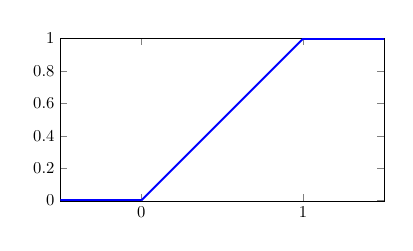
\begin{tikzpicture}[scale = 0.6]
       \begin{axis}[unit vector ratio=1 1 1, ymin=-0.0025,ymax=1.0025,xmin=-0.5, xmax = 1.5, xtick={0,1},ytick={0,0.2,0.4,0.6,0.8,1}]
       \addplot[very thick,domain=-1:0,blue] {0};
       \addplot[very thick,domain=0:1,blue] {x};
       \addplot[very thick,domain=1:2,blue] {1};
    \end{axis}
\end{tikzpicture}
\end{minipage}
\end{center}

Using this cdf, we can determine the probability that $X$ will be in various subsets of $[0,1]$. Let's take the interval $(\frac{2}{5},\frac{2}{3})$. Using the cdf above, we can compute

\begin{center}
    \begin{minipage}{.5\textwidth}
        \centering
        \eqnsgap{P(X \in (\textstyle\frac{2}{5},\frac{2}{3})) &= P(\textstyle\frac{2}{5} < X < \frac{2}{3}) \\
&= P(X < \textstyle\frac{2}{3}) - P(X \leq \frac{2}{5}) \\
&= F_X(\textstyle\frac{2}{3} - ) - F_X(\frac{2}{5}) \\
&= \textstyle \frac{2}{3} - \frac{2}{5} = \frac{4}{15}}
    \end{minipage}%
    \begin{minipage}{0.5\textwidth}
        \centering
    \begin{tikzpicture}[scale = 0.6]
       \begin{axis}[unit vector ratio=1 1 1, ymin=-0.0025,ymax=1.0025,xmin=-0.5, xmax = 1.5, xtick parsed={0,2/5,2/3,1},ytick={0,0.2,0.4,0.6,0.8,1},  xticklabel style={/pgf/number format/frac, /pgf/number format/frac shift=2}]
       \addplot[very thick,domain=-1:0,blue] {0};
       \addplot[name path = f, very thick,domain=0:1,blue] {x};
       \addplot[very thick,domain=1:2,blue] {1};
       \draw[black] (axis cs: 2/3,0) -- (axis cs: 2/3,2/3);
       \draw[black] (axis cs: 2/5,0) -- (axis cs: 2/5,2/5);
    \end{axis}
\end{tikzpicture}
\end{minipage}
\end{center}

\par
\rmk Recall $F_X(a - )$ is shorthand for $\lim_{x \to a^{-}}F_X(x)$, which gives $P(X < a)$. If the cdf of $X$ is continuous, however, as is the case in our example above, then $\lim_{x \to a^{-}}F_X(x) = \lim_{x \to a^{+}}F_X(x) = F_X(a)$, and hence $F_X(a-)$, $F_X(a+)$ and $F_X(a)$ are all equal. When dealing with continuous cdfs we'll simply omit the $-$ or $+$ from now on since it makes no difference in our results.
\par
Note that this implies a random variable $X$ with a continuous cdf will take any fixed real number value with probability zero, since
$$P(X = x) = P(X \leq x) - P(X < x) = F_X(x) - F_X(x-) = 0.$$
It makes sense to ask for the probability that such a random variable falls into a certain range or interval, but the probability it's exactly equal to a given value is always zero. This implies that $P(X \in (a,b))$, $P(X \in [a,b))$, $P(X \in (a,b])$, and $P(X \in [a,b])$ are all equal.
\par
\begin{defn}If $X$ is a random variable whose cumulative distribution function $F_X(x) = P(X \leq x)$ is continuous, then we say $X$ is a continuous random variable.
\end{defn}
\par
\begin{examp}\label{ContinuousCDFExample} Consider the continuous random variable $X$ whose cdf is given below. Find $P(X \in (\frac{1}{3}, 1) \cup [\frac{3}{2}, \frac{5}{2}])$.
\vspace{-1em}
\begin{center}
    \begin{minipage}{.5\textwidth}
        \centering
        \renewcommand*{\arraystretch}{1.35}
\eqns{F_X(x) = \left\{
\begin{array}{cl}
      0 & \text{ if \ } x < 0  \\
      \frac{1}{2}x & \text{ if \ } 0 \leq x < 1  \\
      \frac{1}{2} & \text{ if \ } 1 \leq x < 2 \\ 
      x - \frac{3}{2} & \text{ if \ } 2 \leq x < 3 \\ 
      1 & \text{ if \ } x \geq 3 \\ \end{array}
\right.}
\vspace{1.25em}
\renewcommand*{\arraystretch}{1}
    \end{minipage}%
    \begin{minipage}{0.5\textwidth}
        \centering
    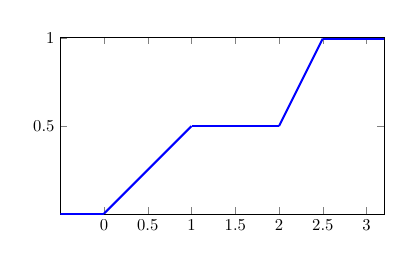
\begin{tikzpicture}[scale = 0.6]
       \begin{axis}[unit vector ratio=1 2 1, ymin=-0.0025,ymax=1.0075,xmin=-0.5, xmax = 3.2, xtick={0,0.5,1,1.5,2,2.5,3},ytick={0.5,1}]
       \addplot[very thick,domain=-1:0,blue] {0};
       \addplot[very thick,domain=0:1,blue] {0.5*x};
       \addplot[very thick,domain=1:2,blue] {0.5};
       \addplot[very thick,domain=2:2.5,blue] {x -1.5};
       \addplot[very thick,domain=2.5:3.3,blue] {1};
    \end{axis}
\end{tikzpicture}
\end{minipage}
\end{center}
\vspace{-1em}
Since the events $X \in (\frac{1}{3}, 1)$ and $X \in [\frac{3}{2}, \frac{5}{2}]$ are mutually exclusive,
 \eqnsgap{P(X \in (\textstyle\frac{1}{3}, 1) \cup [\frac{3}{2},\frac{5}{2}]) &= P(X \in (\textstyle\frac{1}{3}, 1)) + P(X \in [\frac{3}{2},\frac{5}{2}]) \\
&= P(X < 1) - P(X \leq \textstyle\frac{1}{3}) + P(X \leq  \frac{5}{2}) - P(X < \frac{3}{2}) \\
&= F_X(1) - F_X(\textstyle\frac{1}{3}) + F_X( \frac{5}{2}) - F_X(\frac{3}{2}) \\
&= \textstyle\frac{1}{2} - \frac{1}{2}\cdot\frac{1}{3} + (\frac{5}{2} - \frac{3}{2}) - \frac{1}{2} \\
&= \textstyle\frac{1}{2} - \frac{1}{6} + 1 - \frac{1}{2} = \frac{5}{6}.}
\end{examp}

\subsection*{Probability Density Functions}
Consider a continuous random variable $X$, and two real numbers $r$ and $s$. We now know that $P(X = r)$ and $P(X = s)$ are both zero, but we can still ask whether $X$ is more likely to end up `close to' $r$ or `close to' $s$.
\par
We can formalize this by asking for the probability $X$ lies in each of the tiny intervals $(s-\epsilon,\, s + \epsilon)$ and $(r-\epsilon, \,r+ \epsilon)$, for some very small positive number $\epsilon$. For example, consider the random variable $X$ defined in the Example \ref{ContinuousCDFExample} above. Is it more likely this variable takes a value close to $\frac{1}{2}$, or that it takes a value close to $\frac{9}{4}$?

\begin{center}
\begin{tikzpicture}[scale = 1]
       \begin{axis}[unit vector ratio=1 2 1, ymin=-0.0025,ymax=1.0075,xmin=-0.5, xmax = 3.2, xtick parsed ={1/2, 9/4},ytick={0.5,1}, xticklabel style={/pgf/number format/frac, /pgf/number format/frac shift=2, /pgf/number format/frac whole = false}]
       \addplot[very thick,domain=-1:0,blue] {0};
       \addplot[very thick,domain=0:0.38,blue] {0.5*x};
       \addplot[very thick,domain=0.38:0.62,red] {0.5*x};
       \addplot[very thick,domain=0.62:1,blue] {0.5*x};
       \addplot[very thick,domain=1:2,blue] {0.5};
       \addplot[very thick,domain=2:2.13,blue] {x -1.5};
       \addplot[very thick,domain=2.13:2.37,red] {x -1.5};
       \addplot[very thick,domain=2.37:2.5,blue] {x -1.5};
       \addplot[very thick,domain=2.5:3.3,blue] {1};
       \node[label={},circle,fill,inner sep=1pt,red] at (axis cs:0.38,0.19) {};
       \node[label={},circle,fill,inner sep=1pt,red] at (axis cs:0.62,0.31) {};
       \node[label={},circle,fill,inner sep=1pt,red] at (axis cs:2.13,0.63) {};
       \node[label={},circle,fill,inner sep=1pt,red] at (axis cs:2.37,0.87) {};
    \end{axis}
    \draw[thick,red] (2.1,0) node {\small )};
    \draw[thick,red] (1.6,0) node {\small (};
    \draw[red,thick] (1.58,0)  -- (2.12,0);
    \draw[thick,red] (5.35,0) node {\small )};
    \draw[thick,red] (4.85,0) node {\small (};
    \draw[red,thick] (4.83,0)  -- (5.37,0);
\end{tikzpicture}
\end{center}
\vspace{-0.5em}
\par
The probability $X$ lies in the interval $(a,b)$ is $F_X(b) - F_X(a)$, the difference in the value of the cdf at the endpoints. For the cdf shown above, the graph is twice as steep when it's near $\frac{9}{4}$ than it is when it's near $\frac{1}{2}$, and hence this difference is twice as large. Therefore, $X$ is twice as likely to assume values near $\frac{9}{4}$ than it is to assume values near $\frac{1}{2}$.
\par
In general then, the probability $X$ lies close to a given value is proportional to the slope of the cdf at that value, but we know how to measure the slope of any function, with the derivative. Thus, given any $x \in \mathbb{R}$, if we evaluate the derivative of $F_X$ at $x$, the larger the result, the more likely it is that $X$ takes a value very close to $x$. Remember that the probability $X=x$ must be zero for all $x \in \mathbb{R}$, so when we evaluate the derivative of $F_X$ at $x$, the result is not a probability, instead it's known as a probability density, and the derivative of $F_X$ is called the probability density function of $X$. 

\begin{defn}\index{Probability Density Function}\index{Continuous Random Variable!probability density of}If $X$ is a continuous random variable with cdf $F_X$, the probability density function of $X$ is denoted $f_X$ and is defined by $f_X(x) = \frac{d}{dx}{F_X}(x)$.
\end{defn}
\par
The cdf $F_X$ of the continuous random variable $X$ defined in Example \ref{ContinuousCDFExample} above is shown once again on the left, and the corresponding probability density function $f_X$ is on the right. It's standard practice to draw vertical lines on the graph of the probability density function as below. These lines are technically not part of the graph, but can make it easier to read.

\begin{center}
    \begin{minipage}{.5\textwidth}
        \centering
       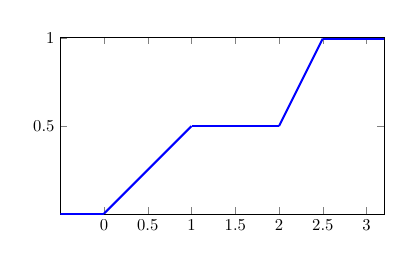
\begin{tikzpicture}[scale = 0.6]
       \begin{axis}[unit vector ratio=1 2 1, ymin=-0.0025,ymax=1.0075,xmin=-0.5, xmax = 3.2, xtick={0,0.5,1,1.5,2,2.5,3},ytick={0.5,1}]
       \addplot[very thick,domain=-1:0,blue] {0};
       \addplot[very thick,domain=0:1,blue] {0.5*x};
       \addplot[very thick,domain=1:2,blue] {0.5};
       \addplot[very thick,domain=2:2.5,blue] {x -1.5};
       \addplot[very thick,domain=2.5:3.3,blue] {1};
    \end{axis}
\end{tikzpicture}
    \end{minipage}%
    \begin{minipage}{0.5\textwidth}
        \centering
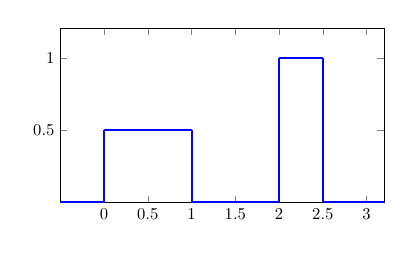
\begin{tikzpicture}[scale = 0.6]
       \begin{axis}[unit vector ratio=1 1.65 1, ymin=-0.0025,ymax=1.2075,xmin=-0.5, xmax = 3.2, xtick={0,0.5,1,1.5,2,2.5,3},ytick={0.5,1}]
       \addplot[very thick,domain=-1:0,blue] {0};
       \addplot[very thick,domain=0:1,blue] {0.5};
       \addplot[very thick,domain=1:2,blue] {0};
       \addplot[very thick,domain=2:2.5,blue] {1};
       \addplot[very thick,domain=2.5:3.3,blue] {0};
       \draw[very thick, blue, -] (axis cs:0,0) -- (axis cs:0,0.5);
       \draw[very thick, blue, -] (axis cs:1,0) -- (axis cs:1,0.5);
       \draw[very thick, blue, -] (axis cs:2,0) -- (axis cs:2,1);
       \draw[very thick, blue, -] (axis cs:2.5,0) -- (axis cs:2.5,1);
    \end{axis}
    \end{tikzpicture}
\end{minipage}
\end{center}

We'll often use pdf to abbreviate probability density function. The rationale for the term `probability density' is the following: when considering a rod of metal or other material, we can only ask for the mass of a contiguous piece of the material, since the mass at a point is always zero. We can, however, consider the density of the material to be well defined at a point, as the rate of change in mass at that point as we move along the rod. The situation with continuous random variables is analogous: a probability density measures the rate of change of the cdf as we move along it, in other words, the rate at which probability is accumulating as we move past that point.
\par
\begin{prop}If $X$ is a continuous random variable, then the probability $X$ lies in the interval $(a,b)$ is the area under $f_X$ on $(a,b)$.
\end{prop}
\begin{pf} Calculating $P(X \in (a,b))$ using the cdf $F_X$ as we have done in the examples above, and applying the fundamental theorem of calculus, we have
$$P(X \in (a,b)) = F_X(b) - F_X(a) = \int_{a}^{b} \frac{d}{dx} F_X(x) \, dx = \int_{a}^{b} f_X(x) \, dx.$$
This integral is the area under $f_X$ on $(a,b)$. Note that the result would be the same with any of the intervals $(a,b]$, $[a,b)$, and $[a,b]$. \end{pf}

\begin{examp} Let X be the continuous random variable whose pdf is given below. Find $P(X > \frac{3}{2})$.
\vspace{-0.5em}
\begin{center}
    \begin{minipage}{.5\textwidth}
        \centering
        \renewcommand*{\arraystretch}{1.35}
\eqns{f_X(x) = \left\{
\begin{array}{cl}
      \frac{2}{x^2} & \text{ if \ } 1 \leq x \leq 2  \\
      0 & \text{ otherwise \ }  \\ \end{array}
\right.}
\vspace{1.25em}
\renewcommand*{\arraystretch}{1}
    \end{minipage}%
    \begin{minipage}{0.5\textwidth}
        \centering
    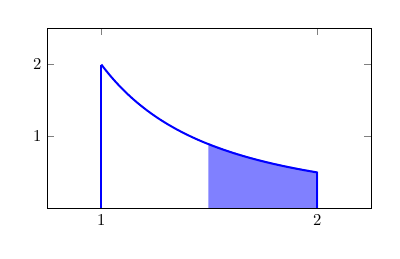
\begin{tikzpicture}[scale =0.6]
       \begin{axis}[unit vector ratio=3 1 1, ymin=-0.0025,ymax=2.5075,xmin=0.75, xmax = 2.25, xtick={1,2},ytick={1,2,3}]
        \addplot[fill = blue, very thick,domain=1.5:2,blue!50, samples=100] {2/(x*x)}\closedcycle;
       \addplot[very thick,domain=1:2,blue, samples=100] {2/(x*x)};
       \draw[very thick, blue, -] (axis cs:1,2) -- (axis cs:1,0);
       \draw[very thick, blue, -] (axis cs:2,0.5) -- (axis cs:2,0);
       \addplot[domain=-3:3] {0};
    \end{axis}
\end{tikzpicture}
\end{minipage}
\end{center}
\vspace{-0.5em}
\eqnsgap{P(X > \textstyle\frac{3}{2}) = \displaystyle\int_{\frac{3}{2}}^{2} f_X(x) \, dx = \int_{\frac{3}{2}}^{2} \frac{2}{x^2} \, dx =  \left.-\frac{2}{x}\,\right|_{\frac{3}{2}}^{2} = -\frac{2}{2} - \left(- \frac{2}{\frac{3}{2}}\right) = \frac{1}{3}}

\end{examp}
\par
\begin{prop}If $X$ is any continuous random variable with cdf $F_X$, the pdf $f_X$ satisfies each of the properties below.
\vspace{-0.5em}
\begin{enumerate}[(i)]
\item For all $x \in \mathbb{R}$, $f_X(x) \geq 0$.
\item $\int_{-\infty}^{\infty} f_X(x) \, dx = P(-\infty < X < \infty) = 1$.
\item $\int_{-\infty}^{t} f_X(x) \, dx = P(X \leq t) = F_X(t)$.
\end{enumerate}
\end{prop}
\par
Intuitively, any non-negative function which encloses an area of one between its graph and the horizontal axis is the pdf of some random variable whose cdf can be recovered through integration, as in $(iii)$ above.

\rmk In fact, the technical details here get difficult and subtle. The mathematical world is teeming with exotic functions which behave in extremely strange ways, but nonetheless this intuition is a good one to have.

\begin{examp}Consider the function $f$ given below. Find $c$ so that this function is the pdf of some continuous random variable.
\renewcommand*{\arraystretch}{1.35}
\eqns{f(x) = \left\{
\begin{array}{cl}
      cxe^{-x} & \text{ if \ } x > 0  \\
      0 & \text{ otherwise \ }  \\ \end{array}
\right.}
\renewcommand*{\arraystretch}{1}
\par
\noindent Since $e^{x}>0$ always, we have $xe^{-x} > 0$ when $x > 0$, and thus $f$ is non-negative when $c > 0$. We must find a positive value for $c$ such that the area under $f$ is one, so we evaluate the area under $f$.
\eqns{\int_{\infty}^{\infty} f(x) \, dx = \int_{0}^{\infty} cxe^{-x} \, dx =c \int_{0}^{\infty} xe^{-x} \, dx =  c(-x-1)e^{-x} \biggr|_{0}^{\infty} }
\par
\noindent The last equality comes from using integration by parts. To complete the evaluation, we can use L'H\^{o}pital's rule.
\eqns{ c(-x-1)e^{-x} \biggr|_{0}^{\infty} &= \lim_{x \to \infty} \left(c(-x-1)e^{-x}\right) - c(-0-1)e^{0}\\
&= c \lim_{x \to \infty} \left( \textstyle\frac{-x-1}{e^{x}}\right) + c \\
&\stackrel{H}{=} c \lim_{x \to \infty} \left( \textstyle\frac{-1}{e^{x}}\right) + c \\
&= 0 + c = c}
\par
\noindent The area under $f$ is simply $c$, and therefore if we take $c=1$, $f$ is a pdf. The graph of $f$ with $c = 1$ is given below.
\begin{center}
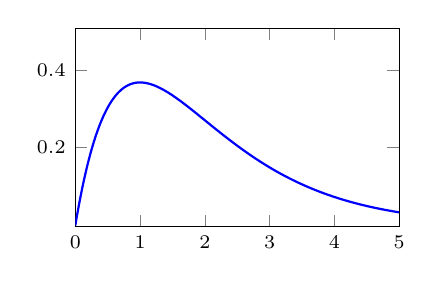
\begin{tikzpicture}
       \begin{axis}[scale = 0.6, unit vector ratio=1 6 1, ymin=-0.0025,ymax=0.5075,xmin=0, xmax = 5, xtick={0,1,2,3,4,5},ytick={0.2,0.4}, tick label style={font=\scriptsize} ]
       \addplot[thick,domain=0:5,blue, samples = 200] {x*(e^(-x))};
    \end{axis}
\end{tikzpicture}
\end{center}
\end{examp}

\subsection*{Functions of a Random Variable}

If $X$ is any random variable and $g: \mathbb{R} \to \mathbb{R}$ is a function, then as we've seen in the discrete case, we can define a new random variable $Y = g(X)$. Given the pdf $f_X$, how can we obtain $f_Y$? Two methods are demonstrated in the examples below, the method of distribution functions and the method of substitution.

\begin{examp}\label{MethodDistributionEx}\index{Method of Distribution Functions}Let $X$ be a real number chosen at random in the interval $[0,2]$, that is, $f_X(x) = \frac{1}{2}$ if $x \in [0,2]$, and $f_X$ is zero otherwise. Find the pdf of $Y = X^2 + 1$ by the method of distribution functions.
\par
\noindent It's not hard to see that the function $F_X$ below is an antiderivative of $f_X$ which goes from zero to one as it progresses along the $x$ axis, and hence is the cdf of $X$.
\renewcommand*{\arraystretch}{1.35}
\eqns{F_X(x) = \left\{
\begin{array}{cl}
      0 & \text{ if \ } x < 0  \\
      \frac{1}{2}x & \text{ if \ } 0 \leq x \leq 2  \\
      1 & \text{ if \ } x > 2  \\ \end{array}
\right.}
\renewcommand*{\arraystretch}{1}
\par
\noindent The functions $f_X$ and $F_X$ are shown below on the left and right respectively.

\begin{center}
    \begin{minipage}{.5\textwidth}
        \centering
        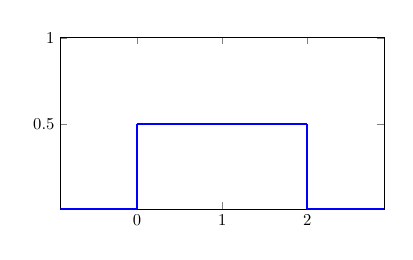
\begin{tikzpicture}[scale = 0.6]
       \begin{axis}[unit vector ratio=1 2 1, ymin=-0.0025,ymax=1.0075,xmin=-0.9, xmax = 2.9, xtick={0,1,2},ytick={0.5,1}]
       \addplot[very thick,domain=-1:0,blue] {0};
       \addplot[very thick,domain=0:2,blue] {0.5};
       \addplot[very thick,domain=2:3,blue] {0};
       \draw[very thick, blue, -] (axis cs:0,0) -- (axis cs:0,0.5);
       \draw[very thick, blue, -] (axis cs:2,0) -- (axis cs:2,0.5);
    \end{axis}
    \end{tikzpicture}
    \end{minipage}%
    \begin{minipage}{0.5\textwidth}
        \centering
        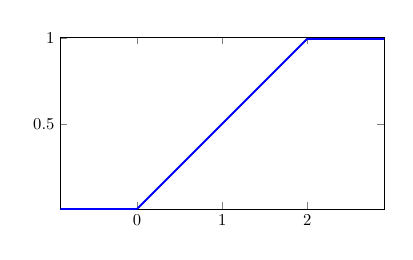
\begin{tikzpicture}[scale = 0.6]
       \begin{axis}[unit vector ratio=1 2 1, ymin=-0.0025,ymax=1.0075,xmin=-0.9, xmax = 2.9, xtick={0,1,2},ytick={0.5,1}]
       \addplot[very thick,domain=-1:0,blue] {0};
       \addplot[very thick,domain=0:2,blue] {0.5*x};
       \addplot[very thick,domain=2:3,blue] {1};
    \end{axis}
\end{tikzpicture}
\end{minipage}
\end{center}
\par
\noindent Now that we have the cdf of $X$, we can use it to determine the cdf of $Y$ as below.
\eqnspar{F_Y(y) = P(Y \leq y) = P(X^2+1 \leq y) = P(X \leq \sqrt{y-1}) = F_X(\sqrt{y-1})}
\par
\noindent Hence if we replace $x$ by $\sqrt{y-1}$ in the cdf of $X$, we obtain the cdf of $Y$. Note that the range of the function $g(x) = x^2+1$ on the interval $[0,2]$ is $[1,5]$, and hence the cdf of $Y$ is given below.
\renewcommand*{\arraystretch}{1.35}
\eqns{F_Y(y) = \left\{
\begin{array}{cl}
      0 & \text{ if \ } y < 1  \\
      \frac{1}{2}\sqrt{y-1} & \text{ if \ } 1 \leq y \leq 5  \\
      1 & \text{ if \ } y > 5  \\ \end{array}
\right.}
\renewcommand*{\arraystretch}{1}
\par
\noindent We now obtain $f_Y(y) = \frac{1}{2}\cdot \frac{1}{2\sqrt{y-1}} = \frac{1}{4\sqrt{y-1}}$ on $[1,5]$ by differentiating the cdf $F_Y$.
\end{examp}
\par
The method of distribution functions is very natural, but its disadvantage is that it requires knowledge of the cdf of $X$. In the example above, it was not difficult to determine $F_X$ from $f_X$, but in general, finding an antiderivative won't always be so easy. We can avoid this issue with the method of substitution.

\begin{examp}\index{Method of Substitution}Let $X$ be a random variable with pdf $f_X(x) = \frac{2}{x^2}$ on $[1,2]$. Find the pdf of $Y = \ln(X)$ by the method of substitution.
\par
\noindent The method of substitution works just like integration by substitution, so it should look familiar. We'll begin with the relationship $y = \ln(x)$, and differentiate to obtain a relationship between the differentials $dy$ and $dx$.
\eqnspar{y = \ln(x) \ \ \rightarrow \ \  dy = \frac{1}{x} \, dx \ \ \rightarrow \ \ dx = x dy \ \ \rightarrow \ \ dx = e^y dy}
\par
\noindent Next, we rewrite $f_X(x) \, dx$ in terms of the variable $y$ and the differential $dy$.
\eqnspar{f_X(x)\, dx = \frac{2}{x^2} \, dx = \frac{2}{({e^y})^2} \, e^y dy = \frac{2}{e^y} \, dy = f_Y(y) \, dy}
\par
\noindent Therefore, $f_Y(y) = \frac{2}{e^y}$ on $[0,\ln(2)]$. As with the last example, we can determine the set of values where $Y$ is nonzero by taking the range of the function $g(x) = \ln(x)$ to the interval $[1,2]$.
\end{examp}
\par
Why does this method work? To develop some intuition for why it does, take for example the random variable $X$ defined by the pdf $f_X(x) = \frac{1}{2}$ on $[0,2]$ and let $Y =X^2+1$, as we did in Example \ref{MethodDistributionEx}.
\par
Consider applying the function $g(x) = x^2+1$ on two different intervals on the horizontal axis. This function sends possible values of $X$ to possible values of $Y$. Let's take two intervals $I = [0.4, 0.6]$ and $J = [1.4,1.6]$ that $X$ might fall into, shown on the left, and consider their images under the function $g(x) = x^2+1$, which are shown on the right.

\begin{center}
    \begin{minipage}{.5\textwidth}
        \centering
\begin{tikzpicture}[scale = 0.6]
       \begin{axis}[unit vector ratio=1 2 1, ymin=-0.0025,ymax=1.0075,xmin=-0.5, xmax = 2.5, xtick parsed ={0,2},ytick={0.5,1}, xticklabel style={/pgf/number format/frac, /pgf/number format/frac shift=2}]
       \addplot[fill = blue, very thick,domain=0.4:0.6,blue!50, samples=100] {0.5}\closedcycle;
       \addplot[fill = blue, very thick,domain=1.4:1.6,blue!50, samples=100] {0.5}\closedcycle;
       \addplot[very thick,domain=-1:0,blue] {0};
       \addplot[very thick,domain=0:2,blue] {0.5};
       \addplot[very thick,domain=2:3,blue] {0};
       \draw[very thick, blue, -] (axis cs:0,0) -- (axis cs:0,0.5);
       \draw[very thick, blue, -] (axis cs:2,0) -- (axis cs:2,0.5);
    \end{axis}
    \draw[thick,red] (2.52,0) node {\small )} node [below right]{$\!I$};
    \draw[thick,red] (2.06,0) node {\small (};
    \draw[red,thick] (2.04,0)  -- (2.54,0);
    \draw[thick,red] (4.34,0) node {\small (};
    \draw[thick,red] (4.80,0) node {\small )} node [below right]{\!$J$};
    \draw[red,thick] (4.32,0)  -- (4.82,0);
\end{tikzpicture}
    \end{minipage}%
    \begin{minipage}{0.5\textwidth}
        \centering
\begin{tikzpicture}[scale = 0.6]
       \begin{axis}[unit vector ratio=1 4 1, ymin=-0.0025,ymax=1.0075,xmin=0, xmax = 6, xtick parsed ={1,5},ytick={0.5,1}, xticklabel style={/pgf/number format/frac, /pgf/number format/frac shift=2}]
       \addplot[fill = blue, very thick,domain=1.16:1.36,blue!50, samples=100] {1/(4*(x-1)^(1/2))}\closedcycle;
       \addplot[fill = blue, very thick,domain=2.96:3.56,blue!50, samples=100] {1/(4*(x-1)^(1/2))}\closedcycle;
       \addplot[very thick,domain=0:1,blue] {0};
       \addplot[very thick,domain=1:5,blue, samples=200] {1/(4*(x-1)^(1/2))};
       \addplot[very thick,domain=5:6,blue] {0};
       \draw[very thick, blue, -] (axis cs:1,0) -- (axis cs:1,1.1);
       \draw[very thick, blue, -] (axis cs:5,0) -- (axis cs:5,0.125);
    \end{axis}
    \draw[thick,red] (1.56,0) node {\small )} node [below right]{\!$g(I)$};
    \draw[thick,red] (1.34,0) node {\small (};
    \draw[red,thick] (1.32,0)  -- (1.58,0);
    \draw[thick,red] (3.38,0) node {\small (};
    \draw[thick,red] (4.09,0) node {\small )} node [below right]{\!$g(J)$};;
    \draw[red,thick] (3.36,0)  -- (4.11,0);
\end{tikzpicture}
\end{minipage}
\end{center}

The events $X \in I$ and $X \in J$ are equally likely, and therefore the events $Y \in g(I)$ and $Y \in g(J)$ must also be, since $Y \in g(I)$ exactly when $X \in I$ and $Y \in g(J)$ exactly when $X \in J$. The values of the pdf $f_Y$ on $g(J)$ are lower than those on $g(I)$, but the intervals have been stretched or squeezed by $g$ so the blue areas are unchanged.
\par
If we interpret $dx$ as a small change in $x$, recall the differential $dy$ approximates the corresponding change in $y$. Here we can imagine $dx$ represents the width of a small interval under the pdf $f_X$, so that $dy$ approximates the width of the image of that interval. This way, the differentials $dx$ and $dy$ account for the stretching and squeezing of the intervals illustrated above.

\section{Expected Value \& Moments}\label{ContinuousMomentsSec}

The expected value of a continuous random variable $X$ is defined in essentially the same way the expected value of a discrete random variable was defined in Section \ref{ExpectedValueSec}. In place of a probability mass function we have a probability density function, and in place of a sum we have the continuous analogue, an integral. We'll also see in this section that all the nice properties of expectation we derived in Section \ref{DiscreteExpectationSec} still hold for continuous random variables.

\begin{defn}\index{Expected Value}\index{Continuous Random Variable!expected value of}
If $X$ is a continuous random variable, the expected value or mean of $X$ is denoted $E(X)$ or $\mu_X$, and defined by the integral below.
\eqns{\boxed{E(X) = \int_{-\infty}^{\infty}x f_X(x) \, dx}}
\par
\noindent Note that this improper integral may not converge, in which case we say that the expected value is undefined.
\end{defn}

\begin{examp}Find the expected value of the random variable $X$ whose pdf is given by $f_X(x) = 2/x^2$ on $[1,2]$.
\eqnsgap{E(X) = \int_{-\infty}^{\infty}x f_X(x) \, dx = \int_{1}^{2}x \,\frac{2}{x^2} \, dx = 2\int_{1}^{2}\frac{1}{x}\, dx = 2 \ln(x) \bigr|_{1}^{2} = 2\ln(2) \\}
\end{examp}

\begin{examp}Consider the random variable $X$ whose pdf is given below (called a Cauchy distribution). Show that $E(X)$ is undefined.
\vspace{-0.75em}
\begin{center}
    \begin{minipage}{.5\textwidth}
        \centering
\eqns{f_X(x) = \frac{1}{\pi(1+x^2)}\text{\ \ on \ }(-\infty,\infty)}
\vspace{1.25em}
    \end{minipage}%
    \begin{minipage}{0.5\textwidth}
        \centering
    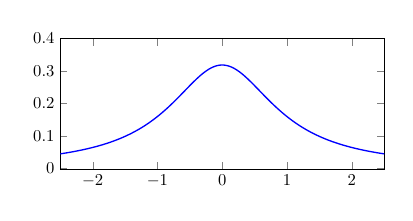
\begin{tikzpicture}[scale=0.6]
       \begin{axis}[unit vector ratio=1 5 1, ymin=-0.0025,ymax=0.4,xmin=-2.5, xmax = 2.5, xtick={-2,-1,0,1,2},ytick={0,0.1,0.2,0.3,0.4}]
       \addplot[thick,domain=-3:3,blue,samples=200] {1/(3.1415*(1+x*x))};
    \end{axis}
\end{tikzpicture}
\end{minipage}
\end{center}
\vspace{-0.5em}
\eqns{E(X) = \int_{-\infty}^{\infty} x f_X(x) \, dx = \int_{-\infty}^{\infty} x \frac{1}{\pi(1+x^2)} \, dx = \frac{1}{\pi}\int_{-\infty}^{\infty} \frac{x}{1+x^2} \, dx}
\par
\noindent To evaluate a `doubly improper' integral like this, we must split it into two improper integrals to see if both of those converge. In the two resulting integrals, we make the substitution $u = 1+x^2$, so $du = 2x \, dx$ and hence $dx = \frac{1}{2x}du$.
\eqns{E(X) &= \frac{1}{\pi}\int_{-\infty}^{\infty} \frac{x}{1+x^2} \, dx \\
&= \frac{1}{\pi}\int_{-\infty}^{0} \frac{x}{1+x^2} \, dx + \frac{1}{\pi}\int_{0}^{\infty} \frac{x}{1+x^2} \, dx \\
&= \frac{1}{\pi}\int_{\infty}^{1} \frac{x}{u} \frac{1}{2x}\, du + \frac{1}{\pi}\int_{1}^{\infty} \frac{x}{u} \frac{1}{2x}\, du \\}
\eqns{\hspace{8.6em}&= \frac{1}{2\pi}\int_{\infty}^{1} \frac{1}{u} \, du + \frac{1}{2\pi}\int_{1}^{\infty} \frac{1}{u} \, du \\ 
&= \frac{1}{2\pi}\ln(u) \biggr|_{\infty}^{1} + \frac{1}{2\pi}\ln(u) \biggr|_{1}^{\infty} \\
&= \frac{1}{2\pi}\left(\ln(1) - \lim_{u \to \infty}ln(u)\right) + \frac{1}{2\pi}\left(\lim_{u \to \infty}ln(u) - \ln(1)\right) \\}
\par
\noindent Neither of the two improper integrals converge since $\lim_{u \to \infty} \ln(u) = \infty$, and hence $E(X)$ is undefined.
\end{examp}

\begin{thm}(Law of the Unconscious Statistician)\index{Law of the Unconscious Statistician} If $X$ is a continuous random variable and $g:\mathbb{R} \to \mathbb{R}$ then the expected value of $Y = g(X)$ is given below.
\eqnsgap{\boxed{E(Y) = \int_{-\infty}^{\infty}g(x)f_X(x)\, dx}}
\end{thm}

\begin{examp}Suppose a 1 metre long stick is broken at a position chosen at random along its length. What is the average length of the longer piece?
\par
\noindent If $X$ denotes the position where the break occurs, then the pdf of $X$ is $f_X(x) = 1$ on $[0,1]$, and the two pieces will have lengths $x$ and $1-x$. The piece of length $x$ is longer when $x > \frac{1}{2}$ and the piece of length $1-x$ is longer when $x < \frac{1}{2}$. Thus, $Y = g(X)$ where
\renewcommand*{\arraystretch}{1.35}
\eqns{g(x) = \left\{
\begin{array}{cl}
      1- x & \text{ if \ } 0 \leq x \leq \frac{1}{2}  \\
      x & \text{ if \ } \frac{1}{2} \leq x \leq 1 \\ \end{array}.
\right.}
\renewcommand*{\arraystretch}{1}
\par
\noindent Now we can calculate the expected value of $Y$ by using the Law of the Unconscious Statistician.
\eqnsbiggap{E(Y) &= \int_{-\infty}^{\infty} g(x) f_X(x) \, dx = \int_{0}^{1} g(x)\cdot 1 \, dx \\
&= \int_{0}^{\frac{1}{2}} g(x) \, dx +  \int_{\frac{1}{2}}^{1} g(x) \, dx \\
&= \int_{0}^{\frac{1}{2}} 1-x \,\, dx +  \int_{\frac{1}{2}}^{1} x \, dx \\
&= (x - \textstyle\frac{1}{2}x^2)\biggr|_{0}^{\frac{1}{2}} + \frac{1}{2}x^2\biggr|_{\frac{1}{2}}^{1}  \\
&= (\textstyle\frac{1}{2} - \frac{1}{8}) - (0 - 0) + \frac{1}{2} - \frac{1}{8} = \frac{3}{4} \\}
Hence, the average length of the longer piece is $\frac{3}{4}$.
\end{examp}
\vspace{0.1em}
\begin{prop}\index{Linearity of Expectation}(Linearity of Expectation) If $X$ and $Y$ are continuous random variables, then $E(aX+b) = aE(X)+b$ and $E(X+Y) = E(X)+E(Y)$.
\end{prop}
\par
In fact, the argument for each of these results in the continuous case mirrors the argument given for the discrete version in Section \ref{ExpectedValueSec}, but everywhere we had a sum, we'll now have an integral. The first property above, for example, can be derived using the Law of the Unconscious Statistician as follows.
\eqns{E(aX+b) &= \int_{-\infty}^{\infty}(ax+b)f_{X}(x)\, dx \\ 
&= \int_{-\infty}^{\infty}axf_{X}(x) + bf_X(x)\, dx \\
&= a\int_{-\infty}^{\infty}xf_{X}(x) \, dx +  b\int_{-\infty}^{\infty}f_X(x)\, dx \\
&= aE(X) + b\cdot 1 = aE(X) + b
}
\par
Compare this to the discrete version, Corollary \ref{LinearityI} in Section \ref{ExpectedValueSec}, and you'll see that it's exactly the same after changing each sum to an integral. For this reason, we'll omit the arguments for the results presented in this section. It's also worth noting that a double sum in the discrete case will become a double integral, and the topic of double integrals deserves a more thorough treatment than we have time for in this course.
\par
The following result comes from such an argument involving double integrals, and can make expected value calculations easier when you have an expression for the cdf of the random variable you're interested in.

\begin{prop}\label{Tail Sum Formula}\index{Tail Sum Formula}\index{Expected Value!tail sum formula for}(Tail Sum Formula) If $X$ is a random variable that takes only non-negative values, then
\eqnsgap{\boxed{E(X) = \int_{0}^{\infty} P(X > x) \, dx = \int_{0}^{\infty} 1- F_X(x) \, dx}}
\end{prop}

\begin{examp}Suppose that $X$ is a randomly selected real number between 1 and 5. Then the pdf of $X$ is $f_X(x) = \frac{1}{4}$ on $[1,5]$, and the cdf of $X$ is given below.
\vspace{-0.75em}
\begin{center}
    \begin{minipage}{.5\textwidth}
        \centering
\renewcommand*{\arraystretch}{1.35}
\eqns{F_X(x) = \left\{
\begin{array}{cl}
      0 & \text{ if \ } x < 1  \\
      \frac{1}{4}(x-1) & \text{ if \ } 1 \leq x < 5  \\
      1 & \text{ if \ } x \geq 5 \\ \end{array}
\right.}
\vspace{1.25em}
\renewcommand*{\arraystretch}{1}
\vspace{0.2em}
    \end{minipage}%
    \begin{minipage}{0.5\textwidth}
        \centering
    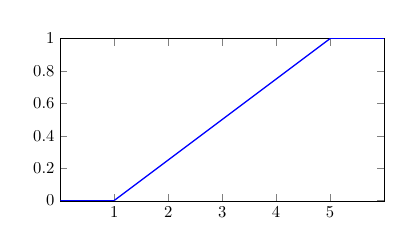
\begin{tikzpicture}[scale=0.6]
       \begin{axis}[unit vector ratio=1 3 1, ymin=-0.0025,ymax=1,xmin=0, xmax = 6, xtick={1,2,3,4,5},ytick={0,0.2,0.4,0.6,0.8,1}]
       \addplot[thick,domain=0:1,blue] {0};
			\addplot[thick,domain=1:5,blue] {0.25*(x-1)};
			\addplot[thick,domain=5:6,blue] {1};
    \end{axis}
\end{tikzpicture}
\end{minipage}
\end{center}
\vspace{-0.5em}
\par
\noindent We can tell that $E(X) = \frac{1+5}{2} = 3$ by symmetry (recall the expected value is the literal balance point of the graph of the pdf). Verify that the tail sum formula yields the same result.
\eqnsgap{E(X) &= \int_{0}^{\infty}1 - F_X(x)\, dx \\
&= \int_{0}^{1} 1 - 0 \ dx + \int_{1}^{5} 1 - \frac{1}{4}(x-1) \, dx  + \int_{5}^{\infty} 1 - 1 \ dx \\
&= \int_{0}^{1} 1 \ dx + \int_{1}^{5} \frac{5}{4}-\frac{1}{4}x \ dx \\
&= x \,\biggr|_{0}^{1} + \left(\frac{5}{4}x-\frac{1}{8}x^2\right)\biggr|_{1}^{5} \\
&= 1 + \left(\frac{25}{4}-\frac{25}{8}\right) - \left(\frac{5}{4} - \frac{1}{8}\right) \\
&= 1+\frac{25}{8}-\frac{9}{8} = 3}
\end{examp}

This example may not convince you the tail sum formula is very helpful, but it should at least provide some evidence that it's correct. We'll see a few examples where the tail sum formula will make our calculations easier in the next few sections.

%If at least 90% of the surface of a sphere is coloured red, show that it's possible to inscribe a cube such that all eight vertices meet the sphere at red coloured points. (Use eight indicator random variables and linearity of expectation)

\subsection*{Variance for Continuous Random Variables}

\begin{defn}\index{Variance}\index{Continuous Random Variable!variance of}The variance of a continuous random variable $X$ is denoted $\Var(X)$ or ${\sigma_X}^2$, and is defined as follows.
\eqns{\boxed{\Var(X) = E[(X - \mu_X)^2] = \int_{-\infty}^{\infty}(x - \mu_X)^2 f_X(x)\, dx}}
\par
\noindent The variance of $X$ is undefined if this improper integral diverges.
\end{defn}
\par
As in the discrete case, the standard deviation of a continuous random variable is defined by $\sigma_X = \sqrt{\Var(X)}$, and the two useful identities below hold. 

\begin{prop}If $X$ is a continuous random variable and $\Var(X)$ is defined, then
\vspace{-2em}
\begin{enumerate}[(i)]
\item $\Var(X) = E[X^2] -(E[X])^2$
\item $\Var(aX+b) = a^2\Var(X)$
\end{enumerate}
\end{prop}

\begin{examp}The proportion of parts produced at a certain factory each day which pass quality control is a random variable with pdf $f_X(x) = 105x^4(1-x)^2$ on $[0,1]$. Find $E(X)$ and $\Var(X)$.
\eqnsgap{E(X) &= \int_{-\infty}^{\infty}xf_X(x)\, dx = \int_{0}^{1}105x^5(1-x)^2\, dx = 105\int_{0}^{1}x^5-2x^6+x^7\, dx \\
&= 105\left(\frac{1}{6}x^6 -\frac{2}{7}x^7 + \frac{1}{8}x^8\right)\biggr|_{0}^{1} = 105\left(\frac{1}{6} -\frac{2}{7} + \frac{1}{8}\right) = 0.625}
\eqnsgap{E(X^2) &= \int_{-\infty}^{\infty}x^2f_X(x)\, dx = \int_{0}^{1}105x^6(1-x)^2\, dx = 105\int_{0}^{1}x^6-2x^7+x^8\, dx \\
&= 105\left(\frac{1}{7}x^7 -\frac{2}{8}x^8 + \frac{1}{9}x^9\right)\biggr|_{0}^{1} = 105\left(\frac{1}{7} -\frac{2}{8} + \frac{1}{9}\right) \simeq 0.4166}
\par
\noindent Thus, $E(X) = 0.625$ and $\Var(X) = E[X^2] - (E[X])^2 \simeq 0.4166 - 0.3906 = 0.0260$. 
\end{examp}
\par
The variance measures the dispersion of a random variable, and so allows to us to compare two random variables on the basis of how much they vary, but so far we haven't been able to make any concrete statements about the values a random variable can take based only on its expected value and variance. The result below allows us to do this by giving a concrete bound on how far a random variable can stray from its expected value.

\begin{thm}(Chebyshev's Inequality)\index{Chebyshev's Inequality}\label{ChebyshevsInequality} For any random variable $X$ whose expected value and variance are defined, the probability that $X$ is within $k$ standard deviations of its expected value is at least $1-\frac{1}{k^2}$. 
\eqnsbiggap{\boxed{P\bigr(X \in (\mu_X - k\sigma_X, \, \mu_X + k\sigma_X)\bigr) \geq 1 - \frac{1}{k^2}}}
\end{thm}
\begin{pf} Consider splitting the integral in the definition of $\Var(X)$ at the endpoints of the interval $(\mu_X - k\sigma_X, \, \mu_X + k\sigma_X)$.
\eqns{\Var(X) &= \int_{-\infty}^{\infty} (x-\mu_X)^2 f_X(x) \, dx \\
&=\int_{-\infty}^{\mu_X - k\sigma_X} (x-\mu_X)^2 f_X(x) \, dx + \int_{\mu_X - k\sigma_X}^{\mu_X + k\sigma_X} (x-\mu_X)^2 f_X(x) \, dx \\ &+ \int_{\mu_X + k\sigma_X}^{\infty} (x-\mu_X)^2 f_X(x) \, dx}
\par
\noindent Note that for the last integral, $x \in (\mu_X + k\sigma_X, \,\infty)$, which means $x > \mu_X + k\sigma_X$, so $(x - \mu_X)^2 > k^2{\sigma_X}^2$. We can make a similar argument if $x \in (-\infty,\, \mu_X + k\sigma_X)$ and conclude $(x - \mu_X)^2 > k^2{\sigma_X}^2$ in that case also. Thus, if we replace $(x-\mu_X)^2$ with $k^2{\sigma_X}^2$ in the first and third integrals, and remove the second integral, whose value must be non-negative since $f_X$ is a non-negative function, we can only have diminished the right hand side.
\eqns{\Var(X) &\geq \int_{-\infty}^{\mu_X - k\sigma_X} k^2{\sigma_X}^2 f_X(x) \, dx + \int_{\mu_X + k\sigma_X}^{\infty} k^2{\sigma_X}^2 f_X(x) \, dx \\
&\geq k^2{\sigma_X}^2 \left(\int_{-\infty}^{\mu_X - k\sigma_X} f_X(x) \, dx + \int_{\mu_X + k\sigma_X}^{\infty} f_X(x) \, dx\right)\\
&\geq k^2{\sigma_X}^2\left[ P\left( X \in (-\infty, \, \mu_X - k\sigma_X) \right)+ P\left( X \in (\mu_X + k\sigma_X, \, \infty) \right)\right]\\
&\geq k^2{\sigma_X}^2\left[ 1 - P\left( X \in (\mu_X - k\sigma_X,\, \mu_X + k\sigma_X)\right)\right]\\}
\par
\noindent Since $\Var(X)={\sigma_X}^2$, dividing both sides by ${\sigma_X}^2$ (which is always positive) yields the inequality below.
\eqns{1 &\geq k^2\left[ 1 - P\left( X \in (\mu_X - k\sigma_X,\, \mu_X + k\sigma_X)\right)\right]\\
\frac{1}{k^2} &\geq  1 - P\left( X \in (\mu_X - k\sigma_X,\, \mu_X + k\sigma_X)\right) \\
-1 + \frac{1}{k^2} &\geq - P\left( X \in (\mu_X - k\sigma_X,\, \mu_X + k\sigma_X)\right) \\
1 - \frac{1}{k^2} &\leq P\left( X \in (\mu_X - k\sigma_X,\, \mu_X + k\sigma_X)\right) \\}
\end{pf}

\begin{examp}\label{ChebyshevEx}On a fishing trip, a fisherman catches ten fish and claims three of them weigh over $10\,kg$. If the average weight of the ten fish is $5.2\,kg$, and the standard deviation is $2.4\,kg$, show that the claim must be false.
\par
\noindent Let $X$ represent the weight of a randomly selected fish in the group of ten, and note that $10 = 5.2+2(2.4)$, so a weight of $10\,kg$ is exactly two standard deviations above the mean. We can use Chebyshev's inequality to determine the minimum number of fish whose weights are within two standard deviations of the mean.
\eqnspar{P\left(X \in (5.2 - 2(2.4),\,5.2+2(2.4)\right) \geq 1 - \frac{1}{2^2} = \frac{3}{4}}
\par
\noindent Thus, at least $75\%$ of the fish must be between $5.2 - 2(2.4) = 0.4\,kg$ and $5.2 + 2(2.4) = 10\,kg$, which means that at most $25\%$ can weigh over $10\,kg$. Three fish over $10\,kg$ would represent a proportion of $30\%$, contradicting Chebyshev's Inequality. Therefore, the claim is false.
\end{examp}
\par
\rmk Note that in Example \ref{ChebyshevEx} above, the random variable $X$, which represents the weight of a randomly selected fish from a certain group of ten, is discrete, since it can only have ten or fewer distinct values. Though the proof was given for the continuous case, Chebyshev's Inequality applies in the discrete case as well.
\par
Chebyshev's Inequality plays an important role in the theoretical foundations of statistics because of its generality. The distribution of $X$ (equivalently, the graph of its pdf $f_X$) might have any ridiculous shape you could imagine, and yet as long as $E(X)$ and $\Var(X)$ are well defined, this inequality gives some simple probabilistic constraints on the value of $X$.

\section{The Uniform Distribution}\label{UniformDistSec}

\begin{defn}\index{Uniform Distribution!continuous}\index{Distribution!Uniform}\index{Uniform Distribution} If the probability density function of $X$ is constant on some interval $I \subseteq \mathbb{R}$, and zero outside $I$, then $X$ is said to be uniformly distributed on the interval I, written $X \sim Uniform(I)$.
\end{defn}
\par
\rmk Be careful not to confuse continuous and discrete uniform distributions. The notation $X \sim Uniform(5)$ describes a discrete random variable that takes values in the set $\{1,2,3,4,5\}$ while $X \sim Uniform([1,5))$ refers to a continuous random variable that takes values in the interval $[1,5)$.
\begin{examp} Let $X$ be uniformly distributed on $[3,7]$. Find $f_X$ and $F_X$.
\par
\noindent To determine $f_X$, we're looking for a positive constant $c$ such that the area under $f_X(x) = c$ on $[3,7]$ is one. This area is a rectangle with width $4$ and height $c$, hence we require $4c = 1$, so $c = \frac{1}{4}$.
\renewcommand*{\arraystretch}{1.35}
\eqns{f_X(x) = \left\{
\begin{array}{cl}
      \frac{1}{4} & \text{ if \ } 3 \leq x \leq 7 \\
      0 & \text{ otherwise }  \end{array}
\right.}
\renewcommand*{\arraystretch}{1}
\par
\noindent To find $F_X$, we have $F_X(x) = \int f_X(x) \,dx = \int \frac{1}{4}\,dx = \frac{1}{4}x + C$ on $[3,7]$, and since $F_X(7) = P(X \leq 7) = 1$, we have $\frac{1}{4}(7) + C = 1$, so $C = -\frac{3}{4}$.
\renewcommand*{\arraystretch}{1.35}
\eqns{F_X(x) = \left\{
\begin{array}{cl}
      0 & \text{ if \ } x < 3 \\
      \frac{1}{4}x - \frac{3}{4} & \text{ if \ } 3 \leq x \leq 7 \\
      1 & \text{ if \ } x > 7  \end{array}
\right.}
\renewcommand*{\arraystretch}{1}
\end{examp}
\vspace{-0.5em}
\par
\noindent In general, if $X$ is uniformly distributed on an interval $I$ which has its left endpoint at $a$ and its right endpoint at $b$, then $f_X(x) = \frac{1}{b-a}$ on $I$ and $f_X$ is zero everywhere else. Next, let's derive the expected value and variance of a continuous uniform random variable.
\par
\begin{prop}\index{Uniform Distribution!expected value of}\index{Uniform Distribution!variance of}\label{UniformVariance}If $I$ is an interval with endpoints $a$ and $b$, and $X \sim Uniform(I)$, then $E(X) = \frac{a+b}{2}$ and $\Var(X) = \frac{1}{12}(b-a)^2$. 
\end{prop}
\begin{pf} We observed above that $f_X(x) = \frac{1}{b-a}$ on $I$, so we calculate $E(X)$ and $E(X^2)$.
\eqns{E(X) = \int_{a}^{b} x f_X(x) \, dx = \int_{a}^{b} x \, \textstyle\frac{1}{b-a} \, dx = \frac{1}{b-a} \displaystyle\int_{a}^{b} x \, dx = \textstyle\frac{1}{b-a}\left(\frac{1}{2}x^2 \bigr|_{a}^{b}\right) = \frac{a+b}{2}}
\eqns{E(X^2) = \int_{a}^{b} x^2 f_X(x) \, dx = \int_{a}^{b} x^2 \, \textstyle\frac{1}{b-a} \, dx = \frac{1}{b-a} \displaystyle\int_{a}^{b} x^2 \, dx = \textstyle\frac{1}{b-a}\left(\frac{1}{3}x^3 \bigr|_{a}^{b}\right) = \frac{a^2+ab+b^2}{3}}
\par
\noindent Note that the difference of squares and difference of cubes identities were used above to simplify the results.
\eqns{\Var(X) = E[X^2] - (E[X])^2 = \textstyle\frac{a^2+ab+b^2}{3} - \frac{a^2+2ab+b^2}{4} = \frac{a^2-2ab+b^2}{12} = \frac{1}{12}(b-a)^2}
\end{pf}
\par Though the uniform distribution is certainly the most basic type of continuous random variable we'll study, there are many interesting problems and applications that involve uniformly distributed quantities. The problem in the introduction to this chapter is a great example.

\begin{examp} Alice and Bob each arrive home from work independently at times uniformly distributed between 5:00\,pm and 6:00\,pm every day. How long, on average, does the person who arrives earlier spend waiting for the one who arrives later?
\par
\noindent In the introduction, we noted that we can represent pairs of arrival times as points in the unit square, Alice's arrival time on the horizontal axis, and Bob's on the vertical axis, both in hours after 5:00\,pm. The waiting time is given by the vertical distance to the diagonal for points above it, and the horizontal distance to the diagonal for points below it. Thus, points in the shaded region shown below on the right occur when Alice and Bob arrive within $x$ hours of each other.

\vspace{-0.5em}
\begin{center}
\begin{minipage}{1.8in}
\centering
\begin{tikzpicture}[scale=0.7]
\node (v1) at (-0.75,0) {};
\fill (v1) circle [radius=2pt];
\node (a) at (-1.8,-1.8) {$0$};
\node (b) at (1.8,-1.8) {$1$};
\node (c) at (-1.8,1.8) {$1$};
\node (l1) at (1.5,1.5) {};
\node (l2) at (-1.5,-1.5) {};
\draw[dotted] (l1.center) -- (l2.center);
\draw(v1.center) -- (-0.75,-0.75);
\draw (-1.5,-1.5) rectangle (1.5,1.5);
\end{tikzpicture}
\end{minipage}
\begin{minipage}{1.8in}
\centering
\begin{tikzpicture}[scale=0.7]
\node (v1) at (-1.5,-1.5) {};
\node (v2) at (-1.5,-0.75) {};
\node (v3) at (0.75,1.5) {};
\node (v4) at (1.5,1.5) {};
\node (v5) at (1.5,0.75) {};
\node (v6) at (-0.75,-1.5) {};
\node (a) at (-1.8,-1.8) {$0$};
\node (b) at (1.8,-1.8) {$1$};
\node (c) at (-1.8,1.8) {$1$};
\node (x) at (-1.15,-1.85) {$x$};
\node (y) at (0.35,-1.85) {$1-x$};
\node(l1) at (-1.5,-1.35) {};
\node(l2) at (-1.5,-1.65) {};
\draw (l1.center) -- (l2.center);
\node(m1) at (-0.75,-1.35) {};
\node(m2) at (-0.75,-1.65) {};
\draw (m1.center) -- (m2.center);
\node(n1) at (1.5,-1.35) {};
\node(n2) at (1.5,-1.65) {};
\draw (n1.center) -- (n2.center);
\draw (v1.center)--(v2.center)--(v3.center)--(v4.center)--(v5.center)--(v6.center);
\fill [pattern=north west lines, pattern color=black] (v1.center)--(v2.center)--(v3.center)--(v4.center)--(v5.center)--(v6.center);
\draw (-1.5,-1.5) rectangle (1.5,1.5);
\end{tikzpicture}
\end{minipage}
\end{center}
\vspace{-0.5em}

\par
\noindent \noindent  If both the $x$ and $y$ coordinates (the arrival times) are uniformly distributed on the axes, the point is uniformly distributed in the square, which has unit area. Thus, the probability that Alice and Bob arrive within $x$ hours of each other is given by the shaded area above, which can be found by subtracting out the areas of the two triangles, to obtain $P(X \leq x) = 1 - 2(\textstyle\frac{1}{2}(1-x)^2) = 1 - (1-x)^2.$
\par
\noindent Thus, $P(X \leq x) = 1 - (1-x)^2$ if $x \in [0,1]$ and $P(X \leq x) = 1$ if $x> 1$. We can now calculate $E(X)$ using the tail sum formula.
\eqns{E(X) &= \int_{0}^{\infty} P(X > x)\, dx = \int_{0}^{1} 1 - P(X \leq x)\, dx = \int_{0}^{1} 1 - (1 - (1-x)^2)\, dx \\
&= \int_{0}^{1} (1-x)^2\, dx = \int_{0}^{1} 1-2x+x^2 \, dx = x - x^2 + \textstyle\frac{1}{3}x^3 \bigr|_{0}^{1} = \frac{1}{3}}
\par
\noindent Thus, the expected waiting time is one third of an hour, or twenty minutes.

\end{examp}

\section{The Exponential Distribution}

\begin{defn}\index{Distribution!Exponential}\index{Exponential Distribution}The random variable $X$ is exponentially distributed with parameter $\lambda > 0$ (often called the rate parameter), written $X \sim Exponential(\lambda)$, if its pdf is given by the function below.

\vspace{-1em}
\begin{center}
    \begin{minipage}{.5\textwidth}
        \centering
      \renewcommand*{\arraystretch}{1.35}
\eqns{f_X(x) = \left\{
\begin{array}{cl}
      \lambda e^{-\lambda x} & \text{ if \ } x \geq 0 \\
      0 & \text{ otherwise }  \end{array}
\right.}
\renewcommand*{\arraystretch}{1}
\vspace{1em}
    \end{minipage}%
    \begin{minipage}{0.5\textwidth}
        \centering
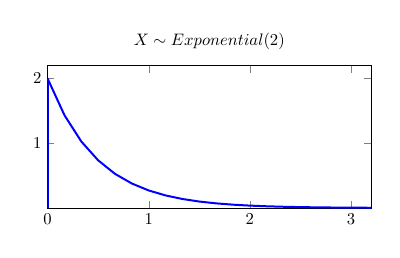
\begin{tikzpicture}[scale = 0.6]
       \begin{axis}[title = {$X \sim Exponential(2)$}, unit vector ratio=1 0.8 1, ymin=-0.0025,ymax=2.2,xmin=-0.0025, xmax = 3.2, xtick = {0,1,2,3}, ytick = {1,2}]
       \addplot[very thick,domain=0:4,blue] {2*e^(-2*x)};
       \draw[very thick, blue, -] (axis cs:0,0) -- (axis cs:0,2);
    \end{axis}
    \end{tikzpicture}
\end{minipage}
\end{center}

\end{defn}
\par
Exponential random variables are used to model time between recurrent events in scenarios where observing such an event gives no information about when the next event will occur. These recurring events are often called arrivals, and the rate parameter $\lambda$ gives the average rate at which the arrivals occur.
\par
Quantities that are typically modelled by exponential random variables include times required for radioactive atoms to decay, distances between mutations on a DNA sequence, and lifetimes of mechanical or electronic devices.
\par
\begin{prop}\index{Exponential Distribution!expected value of}If $X \sim Exponential(\lambda)$, then its cdf is the function given below, and $E(X) = \frac{1}{\lambda}$.
\renewcommand*{\arraystretch}{1.35}
\eqnsgap{F_X(x) = \left\{
\begin{array}{cl}
      0 \ \ \ \ & \text{ if \ } x < 0 \\
      1 - e^{-\lambda x} & \text{ if \ } x \geq 0 \end{array}
\right.}
\renewcommand*{\arraystretch}{1}
\end{prop}
\begin{pf} To obtain the cdf $F_X$, let's find an antiderivative for $f_X$ on $[0, \infty)$ using the substitution $u  = - \lambda x$, so $du = - \lambda dx$, and $dx = \frac{-1}{\lambda} du$.
\eqns{\int f_X(x) \, dx &= \int \lambda e^{-\lambda x} \, dx \\ &= \int \lambda e^{u} \, \frac{-1}{\lambda} \, du \text{ \ where \ } u = -\lambda x  \\ &= - \int e^{u} \, du \\ &= -e^u + C \\ &=  -e^{-\lambda x} + C}
\par
\noindent Thus, $F_X(x) = -e^{-\lambda x} + C$ on $[0,\infty)$, and since $F_X(0) = P(X \leq 0) = 0$, we have $e^{0} + C = 0$, hence $C = 1$ and $F_X(x) = 1 - \lambda e^{-\lambda x}$ as desired. Now, using the tail sum formula,
\eqnspar{E(X) &= \int_{0}^{\infty} 1 - F_X(x) \, dx \\ &= \int_{0}^{\infty} 1 - (1-e^{-\lambda x}) \, dx \\ &= \int_{0}^{\infty} e^{-\lambda x}\, dx  \\ &= \int_{0}^{-\infty} e^{u} \frac{-1}{\lambda}\, du  \text{ \ where \ } u = -\lambda x  \\ &= \frac{-1}{\lambda}\int_{0}^{-\infty} e^{u} \, du \\ &= \frac{-1}{\lambda}\left(\lim_{u \to -\infty} e^u - e^{0}\right) \\ &= \frac{-1}{\lambda}\left(0 - 1\right) = \frac{1}{\lambda}.}
\end{pf}
\begin{examp}At a certain intersection, there is an average of three car accidents per day. Assuming the time between crashes is exponentially distributed, what is the probability that the next two accidents will occur at least five hours apart?
\par
\noindent Let $X$ denote the gap between consecutive crashes in hours. Then $X$ is exponentially distributed and $E(X) = \frac{1}{\lambda} = 8$ since there is an average of $3$ crashes in $24$ hours, so the average gap between crashes is $8$ hours. Thus, $\lambda = \frac{1}{8}$. Note that we can also interpret this as a rate, one crash per eight hours on average. 
\eqnsgap{P(X \in (5,\infty)) &= 1- \int_{0}^{5} f_X(x) \, dx  \\ &= 1 - \int_{0}^{5} \frac{1}{8}e^{-\frac{1}{8}x}\,dx \\ &= 1 - \int_{0}^{-\frac{5}{8}}\frac{1}{8}e^{u}(-8\, du)  \text{ \ where \ } u = -\frac{1}{8} x  \\ &= 1+\int_{0}^{-\frac{5}{8}}e^u \, du \\ &= 1 + \left( e^u \bigr|_{0}^{-\frac{5}{8}}\right) \\ &= 1 + (e^{-\frac{5}{8}} - 1) \simeq 0.535}
\end{examp}
\par
The variance of an exponential random variable can be derived from the formula $\Var(X) = E[X^2] - (E[X])^2$ after computing $E[X^2]$ using integration by parts. The result is given below, and the proof is left as an exercise.
\begin{prop}\index{Exponential Distribution!variance of} If $X \sim Exponential(\lambda)$, then $\Var(X) = \frac{1}{\lambda^2}$.
\end{prop}
\par
One key property of the exponential distribution is that it's `memoryless'. If $X$ is an exponentially distributed random variable representing, for example, a gap between recurring events, then regardless of how long you've already been waiting for the next event to occur, the probability that it will occur in the next minute is the same. Formally, we can state the memoryless property as follows.
\begin{prop} (Memoryless Property)\index{Exponential Distribution!memoryless property of}\index{Memoryless Property} If $X$ is an exponentially distributed random variable, and $a,b \in \mathbb{R}$, then $P(X > a+b \given X>b) = P(X > a)$.
\end{prop}
\begin{examp} Suppose that the lifetime of a certain model of monitor is exponentially distributed, with an average of ten years. If one of these monitors has already lasted fifteen years, what is the probability it will last at least five more years?
\par
\noindent To show the memoryless property holds, we'll calculate $P(X > 20 \given X > 15)$, and then check that we would obtain the same result with $P(X > 5)$. Since the average lifetime is ten years, we have $E(X) = \frac{1}{\lambda} = 10$, hence $\lambda = \frac{1}{10}$. 
\eqns{P(X > 20) &= 1 - P(X \leq 20) = 1 - (1 - e^{-\frac{1}{10} \cdot 20}) = e^{-2} \\
P(X > 15) &= 1 - P(X \leq 15) = 1 - (1 - e^{-\frac{1}{10} \cdot 15}) = e^{-\frac{3}{2}}}
\eqns{P(X > 20 \given X > 15) = \displaystyle\frac{P(X > 20 \cap X > 15)}{P(X > 15)} = \frac{P(X > 20)}{P(X > 15)} = \frac{e^{-2}}{e^{-\frac{3}{2}}}= e^{-\frac{1}{2}}}
\par
\noindent The probability the monitor will last at least five more years is $e^{-\frac{1}{2}} \simeq 0.607$, and the memoryless property states that we'll obtain the same result by simply calculating 
\eqns{P(X>5) = 1 - P(X \leq 5) = 1 - (1 - e^{-\frac{1}{10} \cdot 5}) = e^{-\frac{1}{2}}.}
\end{examp}

\section{The Pareto Distribution}

\begin{defn}\index{Distribution!Pareto}\index{Pareto Distribution}The random variable $X$ is Pareto distributed with the two parameters $m > 0$ (the minimum) and $c > 0$ (often called the shape parameter), written as $X \sim Pareto(m,c)$, if its pdf is given by the function below.

\vspace{-1em}
\begin{center}
    \begin{minipage}{.5\textwidth}
        \centering
      \renewcommand*{\arraystretch}{1.35}
\eqnspar{f_X(x) = \left\{
\begin{array}{cl}
      \frac{cm^c}{x^{c+1}} & \text{ if \ } x \geq m \\
      0 & \text{ otherwise }  \end{array}
\right.}
\renewcommand*{\arraystretch}{1}
\vspace{1em}
    \end{minipage}%
    \begin{minipage}{0.5\textwidth}
        \centering
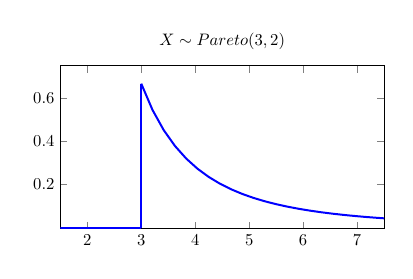
\begin{tikzpicture}[scale = 0.6]
       \begin{axis}[title = {$X \sim Pareto(3,2)$}, unit vector ratio=1 4 1, ymin=-0.005,ymax=0.75,xmin=1.5, xmax = 7.5, xtick = {2,3,4,5,6,7}, ytick = {0.2,0.4,0.6}]
       \addplot[very thick,domain=3:8,blue] {(18)/x^3};
       \draw[very thick, blue, -] (axis cs:3,0) -- (axis cs:3,18/27);
       \draw[very thick, blue, -] (axis cs:1.5,0) -- (axis cs:3,0);
    \end{axis}
    \end{tikzpicture}
\end{minipage}
\end{center}
\end{defn}

\par
This distribution is named for Italian engineer and economist Vilfredo Pareto, who noted that 80\% of land in Italy was owned by 20\% of the population. If we extend this idea further and imagine that of those 20\% who own the most land, 80\% of the land they own is held by the top 20\% of them, and so on, then the distribution of the amount of land owned by a randomly selected Italian individual will be well approximated by a Pareto random variable. This `80-20 rule' or similar proportionality rules appear in many contexts, and when they do the Pareto distribution is typically involved.
\par
Pareto distributions have been used to model household income, sizes of cities (by population), magnitudes of earthquakes, and sizes of insurance claims. %http://www-personal.umich.edu/~mejn/courses/2006/cmplxsys899/powerlaws.pdf
\par
\begin{examp} If the population of a randomly selected US city is approximated by a Pareto distributed random variable $X \sim Pareto(40\,000,2.3)$, what proportion of cities have a population between 100\,000 and 1\,000\,000?
\eqnsgap{P(100\,000 < X <1\,000\,000) &= \int_{100\,000}^{1\,000\,000} \frac{2.3 \cdot 40\,000^{\,2.3}}{x^{3.3}} \,dx  \\ &= 2.3\cdot 40\,000^{\,2.3}\int_{100\,000}^{1\,000\,000} \frac{1}{x^{3.3}} \, dx \\ &= 2.3\cdot 40\,000^{\,2.3} (\textstyle\frac{-1}{2.3}x^{-2.3})\bigr|_{1}^{100} \\&= -40\,000^{\,2.3} (x^{-2.3})\bigr|_{1}^{100} \simeq 12.1\%}
\end{examp}
\begin{prop}\index{Pareto Distribution!expected value of} If $X \sim Pareto(m,c)$, then $E(X) = \frac{cm}{c-1}$ if $c > 1$, and $E(X)$ is undefined if $c \leq 1$.
\end{prop}
\begin{pf} Let $X \sim Pareto(m,c)$, then
\eqns{E(X) &= \int_{\infty}^{\infty}xf_X(x) \, dx = \int_{m}^{\infty}x\frac{cm^c}{x^{c+1}} \, dx = cm^c\int_{m}^{\infty}\frac{1}{x^{c}} \, dx \\ &= cm^c \frac{-1}{(c-1)}x^{-(c-1)} \biggr|_{m}^{\infty} = \frac{cm^c}{c-1}\left(-\left( \lim_{x \to \infty}\frac{1}{x^{c-1}}\right) + \frac{1}{m^{c-1}}\right).}
\par
\noindent Note that the argument above does not apply if $c = 1$, since when we integrate $\frac{1}{x}$, we would obtain $\ln(x)$. However, if $c \neq 1$, we obtain the expression above, and the value of the resulting limit depends only on whether the exponent on $x$ is positive or negative.
\eqns{\lim_{x \to \infty}\frac{1}{x^{c-1}}= \left\{
\begin{array}{cl}
      0 & \text{ if \ } c > 1 \\
      \infty & \text{ if \ } c < 1 \end{array}
\right.}
\renewcommand*{\arraystretch}{1}
\par
\noindent Thus, $E(X)$ is undefined if $c<1$, and $E(X) =  \frac{cm^c}{c-1}\left(\frac{1}{m^{c-1}}\right) = \frac{cm}{c-1}$ if $c >1$. We need to deal with the case $c=1$ separately.
\eqns{E(X) &= \int_{\infty}^{\infty}xf_X(x) \, dx = \int_{m}^{\infty}x\frac{1\cdot m^1}{x^{2}} \, dx = m\int_{m}^{\infty}\frac{1}{x} \, dx \\ &= m\ln(x) \biggr|_{m}^{\infty} = m\left(\left(\lim_{x \to \infty} \ln(x)\right) - \ln(m)\right) \to \infty}
\end{pf}

We can determine $E(X^2)$ by a very similar calculation. Applying the formula $\Var(X^2) = E[X^2] - (E[X])^2$ yields the result below.

\begin{prop}\label{ParetoVariance}\index{Pareto Distribution!variance of}If $X \sim Pareto(m,c)$, then $\Var(X) = \frac{cm^2}{(c-1)^2(c-2)}$ if $c>2$, and $\Var(X)$ is undefined if $c \leq 2$.\end{prop}

\begin{examp} Suppose that a Pareto distribution is used to model a quantity with an average value of $4$ and a variance of $2$. What are the parameters $m$ and $c$?
\par
\noindent Since $E(X) = 4$, we have $4 = \frac{cm}{c-1}$, so $c-1 = \frac{cm}{4}$. Substituting this result into the variance formula given in Proposition \ref{ParetoVariance} above,
\eqns{2 &= \frac{cm^2}{(c-1)^2(c-2)} = \frac{cm^2}{\frac{c^2m^2}{16}(c-2)} = \frac{16}{c(c-2)}}
\par
\noindent Cross-multiplying and solving the resulting quadratic, $2c(c-2) = 16$, the positive solution is $c = 4$, which we can substitute back into $4 = \frac{cm}{c-1}$ to obtain
\eqns{4 = \frac{m \cdot 4}{3}  \ \ \rightarrow \ \ m = 3.}

\end{examp}

%\begin{examp} If $X \sim Exponential(\lambda)$, show that $Y = e^{X}$ is Pareto distributed. What are the parameters of $Y$?
%\par
%\noindent Using the method of substitution, $y = e^x$ implies $dy = e^x \, dx$ and $dx = \frac{1}{y}\, dy$, so
%\eqns{f_X(x) \, dx &= \lambda e^{-\lambda x} \, dx = \lambda (e^{x})^{-\lambda} \frac{1}{y} \, dy = \lambda (e^{\ln(y)})^{-\lambda} \frac{1}{y} \, dy \\ &= \lambda y^{-\lambda} \frac{1}{y} \, dy = \frac{\lambda}{y^{\lambda+1}} \, dy = \frac{\lambda (1)^{\lambda}}{y^{\lambda + 1}}\, dy = f_Y(y)\, dy.}
%\par
%\noindent If $x \in [0,\infty)$, then $y \in [1,\infty)$, so $f_Y(y) = \frac{\lambda (1)^{\lambda}}{y^{\lambda + 1}}$ on $[1,\infty)$. Therefore, $Y$ is pareto distributed with $m = 1$ and $c = \lambda$.
%\end{examp}

\section{The Normal Distribution}

\begin{defn}\index{Distribution!Normal}\index{Distribution!Gaussian}\index{Normal Distribution}\index{Gaussian Distribution}The random variable $X$ is normally distributed with parameters $\mu$ (the mean) and $\sigma > 0$ (the standard deviation) if its pdf is given by the function below on the interval $(-\infty,\infty)$.
\renewcommand*{\arraystretch}{1.35}
\eqnspar{f_X(x) = \frac{1}{\sqrt{2\pi\sigma^2}}\, e^{-\frac{(x-\mu)^2}{2\sigma^2}}}
\renewcommand*{\arraystretch}{1}

\begin{center}
    \begin{minipage}{.5\textwidth}
        \centering
  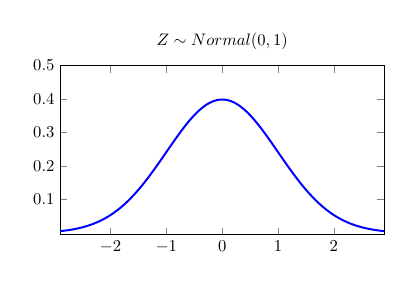
\begin{tikzpicture}[scale = 0.6]
       \begin{axis}[title = {$Z \sim Normal(0,1)$}, unit vector ratio=1 6 1, ymin=-0.005,ymax=0.5,xmin=-2.9, xmax = 2.9, xtick = {-2,-1,0,1,2}, ytick = {0.1,0.2,0.3,0.4,0.5}]
       \addplot[very thick,domain=-3:3,blue, samples=100] {0.3989*e^(-x^2/2)};
    \end{axis}
    \end{tikzpicture}
    \end{minipage}%
    \begin{minipage}{0.5\textwidth}
        \centering
  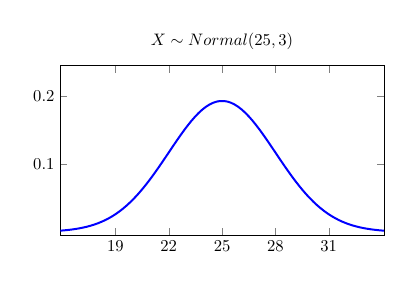
\begin{tikzpicture}[scale = 0.6]
       \begin{axis}[title = {$X \sim Normal(25,3)$}, unit vector ratio=1 38.2 1, ymin=-0.005,ymax=0.245,xmin=15.9, xmax = 34.1, xtick = {19,22,25,28,31}, ytick = {0.1,0.2,0.3,0.4,0.5}]
       \addplot[very thick,domain=15:35,blue, samples =100] {0.19298*e^(-(x-25)^2/18)};
    \end{axis}
    \end{tikzpicture}
\end{minipage}
\end{center}

\end{defn}
\par
This is also referred to as the Gaussian distribution, after mathematician Carl Friedrich Gauss. It will play a central role in the theory of statistics we'll develop in the next few chapters. 
\par
\rmk Unfortunately, the pdf $f_X$ for the normal distribution is not integrable in elementary terms. In other words, its antiderivative can't be expressed using only the functions and operations you've encountered in Cal II, which is a big problem, as it means we can't find areas under the curve using those methods.
\par
The traditional way to get around this problem is to use a large table of values. Unless otherwise stated, the letter $Z$ will be reserved for the random variable $Z \sim Normal(0,1)$ from now on, and a $Z$-table is simply a large table of values of the cdf $F_Z(z) $, that is, the area to the left of $z$, for various $z \in \mathbb{R}$.
\par
What if $X$ is a normally distributed random variable with a mean which is not zero and a standard deviation which is not one? As you might expect given the two graphs above, any two normal distributions differ by shifting and scaling, in the following precise sense.
\begin{prop}$X \sim Normal (\mu,\sigma)$, then $Z = \frac{X - \mu}{\sigma} \sim Normal(0,1)$.
\end{prop}
\begin{pf}
Using substitution, let $z = \frac{x - \mu}{\sigma} = \frac{1}{\sigma}x - \frac{\mu}{\sigma}$, so $dz = \frac{1}{\sigma}\,dx$, and $dx = \sigma \, dz$. 
\eqns{f_X(x)\,dx &= \frac{1}{\sqrt{2\pi\sigma^2}}\, e^{-\frac{(x-\mu)^2}{2\sigma^2}} \, \sigma \, dz \\ &= \frac{1}{\sigma\sqrt{2\pi}}\, e^{-\frac{(\mu+\sigma z-\mu)^2}{2\sigma^2}} \, \sigma \, dz \\ &= \frac{1}{\sqrt{2\pi}}e^{-\frac{z^2}{2}}\, dz = f_Z(z) \, dz}
\par
\noindent Thus, $f_Z$ is the pdf of a normal distribution with $\mu = 0$ and $\sigma = 1$ as claimed.
\end{pf}
\par
The process of translating values of any normally distributed random variable into corresponding values of $Z$ is known as standardization\index{Standardization}. To standardize a value $x$ of a normally distributed random variable $X \sim Normal(\mu, \sigma)$ we simply apply the formula $z  = \frac{x - \mu}{\sigma}$, and we can treat the resulting $z$ as a value of $Z \sim Normal(0, 1)$.
\begin{examp}\label{FemaleHeightsNormal} The height of a randomly selected Canadian adult female, in inches, is approximated by the random variable $X \sim Normal(64,2.5)$. What proportion of Canadian adult females are taller than 5'8"? What proportion have heights between 5'3" and 5'7"?
\par
\noindent To standardize 5'8"\,=\,68", we calculate $z = \frac{68 - 64}{2.5} = 1.6$. Then we have
\vspace{-1em}
\begin{center}
    \begin{minipage}{.5\textwidth}
        \centering
  \eqns{P(X > 68) &= P(Z > 1.6) \\ &= 1 - P(Z \leq 1.6) \\ &= 1 - 0.9452 \\ &= 0.0548 \simeq 5.5\%.}
  \vspace{1.25em}
    \end{minipage}%
    \begin{minipage}{0.5\textwidth}
        \centering
   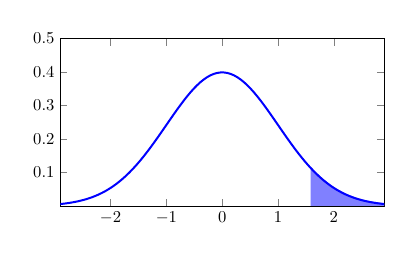
\begin{tikzpicture}[scale = 0.6]
       \begin{axis}[unit vector ratio=1 6 1, ymin=0,ymax=0.5,xmin=-2.9, xmax = 2.9, xtick = {-2,-1,0,1,2}, ytick = {0.1,0.2,0.3,0.4,0.5}]
       \addplot[fill = blue, very thick,domain=1.6:3,blue!50, samples=100] {0.3989*e^(-x^2/2)}\closedcycle;
       \addplot[very thick,domain=-3:3,blue, samples=100] {0.3989*e^(-x^2/2)};
       \addplot[domain=-3:3] {0};
    \end{axis}
    \end{tikzpicture}
\end{minipage}
\end{center}

\par
\noindent Thus, about 5.5\% of Canadian adult females are taller than 5'8". For the second part we standardize 5'3"\,=\,63" and 5'7"\,=\,67" to obtain $z_1 = \frac{63-64}{2.5} = -0.4$ and $z_2 = \frac{67-64}{2.5} = 1.2$, then calculate
\vspace{-1em}
\begin{center}
    \begin{minipage}{0.5\textwidth}
        \centering
  \eqns{P(63 < X < 67) &= P(-0.4 < Z < 1.2) \\ &= P(Z \leq 1.2) - P(Z \leq -0.4) \\ &= 0.8849 - 0.3446 \\ &= 0.5404 \simeq 54\%.}
  \vspace{1.25em}
    \end{minipage}\begin{minipage}{0.5\textwidth}
        \qquad\qquad\centering
   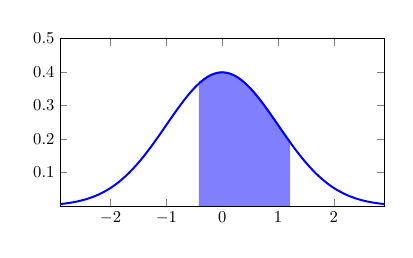
\begin{tikzpicture}[scale = 0.6]
       \begin{axis}[unit vector ratio=1 6 1, ymin=0,ymax=0.5,xmin=-2.9, xmax = 2.9, xtick = {-2,-1,0,1,2}, ytick = {0.1,0.2,0.3,0.4,0.5}]
       \addplot[fill = blue, very thick,domain=-0.4:1.2,blue!50, samples=100] {0.3989*e^(-x^2/2)}\closedcycle;
       \addplot[very thick,domain=-3:3,blue, samples=100] {0.3989*e^(-x^2/2)};
       \addplot[domain=-3:3] {0};
    \end{axis}
    \end{tikzpicture}
\end{minipage}
\end{center}

\par
\noindent Therefore, around 54\% of Canadian adult females are between 5'3" and 5'7".
\end{examp}
\par
Nowadays, we have easy access to computers which can calculate areas under the pdf of $Z \sim Normal(0,1)$ efficiently using numerical integration, so the $Z$-table is something of a mathematical artifact whose uses are limited to classrooms and standardized tests.

\subsection*{Normal Distribution Shortcuts}

Any normal distribution has two inflection points, and these points occur exactly one standard deviation from the mean. This fact is useful when drawing a quick sketch of a normal distribution.
\begin{center}
  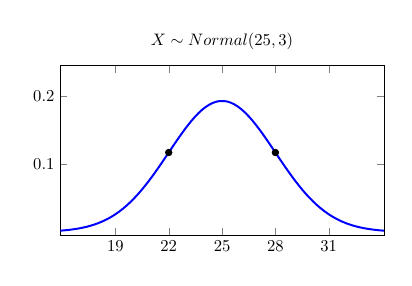
\begin{tikzpicture}[scale = 0.6]
       \begin{axis}[title = {$X \sim Normal(25,3)$}, unit vector ratio=1 38.2 1, ymin=-0.005,ymax=0.245,xmin=15.9, xmax = 34.1, xtick = {19,22,25,28,31}, ytick = {0.1,0.2,0.3,0.4,0.5}]
       \addplot[very thick,domain=15:35,blue, samples =100] {0.19298*e^(-(x-25)^2/18)};
       \addplot [only marks] table {
28 0.11704
22 0.11704
};
    \end{axis}
    \end{tikzpicture}
 \end{center}
\par
For approximate reasoning about normally distributed quantities without the aid of a $Z$-table or computer, the proposition below presents a well-known rule of thumb.
\begin{prop}\index{68-95-99.7 Rule}\label{NormalRuleThumb}(68-95-99.7 Rule) For any normal distribution, 68\% of the area under its pdf occurs within one standard deviation of the mean, 95\% occurs within two standard deviations, and 99.7\% occurs within three standard deviations.
\begin{center}
  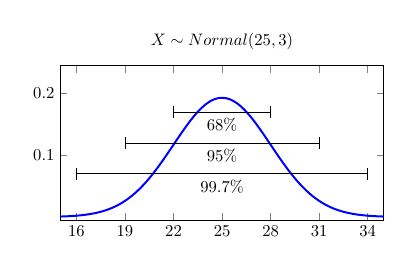
\begin{tikzpicture}[scale = 0.6]
       \begin{axis}[title = {$X \sim Normal(25,3)$}, unit vector ratio=1 38.2 1, ymin=-0.005,ymax=0.245,xmin=15, xmax = 35, xtick = {16,19,22,25,28,31,34}, ytick = {0.1,0.2,0.3,0.4,0.5}]
       \addplot[very thick,domain=15:35,blue, samples =100] {0.19298*e^(-(x-25)^2/18)};
       \draw (axis cs:22,0.17) -- node[below]{68\%} (axis cs:28,0.17);
       \draw (axis cs:19,0.12) -- node[below]{95\%} (axis cs:31,0.12);
       \draw (axis cs:16,0.07) -- node[below]{99.7\%} (axis cs:34,0.07);
       \draw (axis cs:22,0.18) -- (axis cs:22,0.16);
       \draw (axis cs:28,0.18) -- (axis cs:28,0.16);
       \draw (axis cs:19,0.13) -- (axis cs:19,0.11);
       \draw (axis cs:31,0.13) -- (axis cs:31,0.11);
       \draw (axis cs:16,0.06) -- (axis cs:16,0.08);
       \draw (axis cs:34,0.06) -- (axis cs:34,0.08);
    \end{axis}
    \end{tikzpicture}
 \end{center}
\end{prop}
\par
As well as being a useful rule of thumb for quick approximate calculations, the rule also illustrates how quickly the distribution decays when it moves away from the mean. For an arbitrary random variable, Chebyshev's Inequality implies that values less than two standard deviations from the mean must occur at least $1-\frac{1}{2^2} = 75\%$ of the time, so values more than two standard deviations from the mean can occur up to $25\%$ of the time. By the 68-95-99.7 Rule above, such values occur only 5\% of the time in a normal distribution. In this sense, normally distributed quantities are very much concentrated around the mean.

\begin{examp}If $X \sim Normal(64,2.5)$ is used to model the height of a randomly selected Canadian female, provide a range of heights which will include 95\% of all Canadian adult females.
\par
\noindent Using the 68-95-99.7 Rule, $95\%$ of Canadian adult females will have heights within two standard deviations of the mean height, 64". So we calculate $64 - 2(2.5) = 59$ and $64 + 2(2.5) =69$. Therefore, 95\% of all Canadian adult females are taller than 59"\,=\,4'11" and shorter than 69"\,=\,5'9".
\end{examp}
